\section{Critical Review}
\captionsetup[figure]{font=small,labelfont=bf}
% Dit hoofdstuk is een opsomming van dat wat er al bekend is over het in de introductie beschreven onderwerp. Zeker bij practice based research gaat dit niet alleen om academische literatuur. Ook repertoire in de vorm van al bestaand werk, maakprocessen, contexten, technologieën, enzovoort is relevant, net als literatuur die niet strict academisch is zoals artikelen uit vakbladen, documentaires, enzovoort. In het critical review hoofdstuk wordt het eerder geïntroduceerde onderwerp in verband gebracht met relevante literatuur en repertoire.

% NOTES
% - Critical review naar bestaande media (Phonograph, LP, tape, CD, MP3, Torrent/P2P, Streaming)
% - Korte technische uitleg wat het is
% - Disruptieve werking van een medium op zijn voorganger
% - Welk probleem heeft het proberen op te lossen

% Inleiding
In dit critical review zal ik een onderzoek doen naar bestaande media en diensten voor muziekdistributie. Hierbij zal worden beschreven wat de disruptieve werking was van het medium ten opzichte van zijn voorganger en wat het probleem is wat het medium probeerde op te lossen. Tot slot zal worden beschreven waarom het medium relevant is voor dit Supportive Narrative en het onderliggende project, de NichePlayer.

% Uitleggen disruptief effect
Onder disruptieve werking versta ik het volgende. Nieuwe media worden vaak uitgevonden in een actie-reactie proces. In het oude medium blijkt na gebruik een tekortkoming te zitten, wat door middel van het nieuwe medium wordt opgelost. Dit proces is niet altijd intentioneel. Sommige innovaties in de geschiedenis hebben geleid tot een grotere hoeveelheid piracy, veranderingen in de muziek zelf, en hoe men ernaar luistert. Positieve effecten zijn bijvoorbeeld het ontstaan van nieuwe genres.

% ---------------------------------------------------------------------------------------- %
\subsection{Analyse bestaande media}
In dit onderzoek kan in theorie terug worden gegaan tot in de oudheid. Het doorgeven en distribueren van muziek is een onderdeel van cultuur, en daarmee iets wat ons mens maakt. Om een kader te stellen wordt gefocust op distributiemedia die klinkend geluid (i.e. geluidsgolven) dragen, beginnende bij de fonograaf.

\subsubsection*{Fonograaf}
\begin{wrapfigure}{r}{0.25\textwidth}
    \centering
    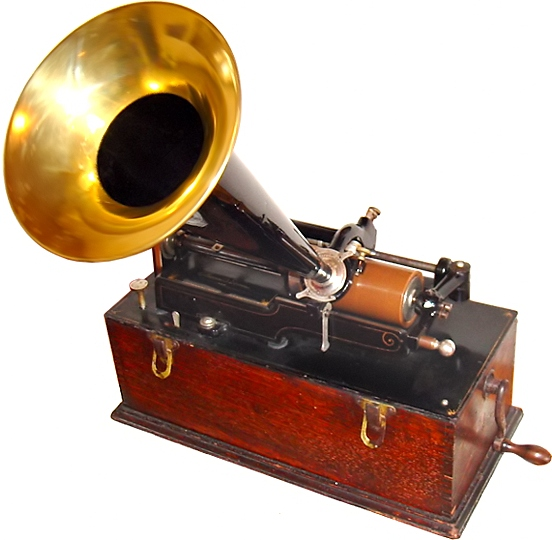
\includegraphics[width=0.25\textwidth]{assets/critical-review/EdisonPhonograph.jpg}
    \caption{Fonograaf}
    \label{fig:critical-review:phonograph}
\end{wrapfigure}

% Beschrijving medium
De fonograaf (phonograph in Engels) is een van de eerste distributie media die het geluid zelf draagt ten opzichte van een beschrijving van de muziek. De geluidsgolven worden opgeslagen door met een naald in een wassen rol te krassen. De diepte van de kras staat gelijk aan de uitslag van het membraan. Tijdens het afspelen wordt het proces omgedraaid; een naald glijdt door de krassen en brengt hiermee het membraan in beweging. Het geluid wordt vervolgens versterkt door een hoorn.

% Klinkende muziek in huis zonder instrument
Door de uitvinding van de fonograaf werd het mogelijk om klinkende muziek in huis te hebben, zonder dat hier een instrument voor bespeeld hoefde te worden. Hiermee werd het dus ook mogelijk om een opname van een heel orkest af te spelen binnen huis, iets wat voor de uitvinding niet mogelijk was. Voor de uitvinding van de fonograaf was het enige alternatief om naar een live concert te gaan. Hoewel de fonograaf best veel geld kostte (rond \$150 in het begin \citep{historyofphonograph}) bracht het een nieuwe mogelijkheid voor normale burgers om naar muziek te luisteren.

% Minder focus op eigen interpretatie
Mensen konden hiermee ook 'perfecte' versies van de muziek beluisteren. In plaats van eigen interpretaties van bladmuziek wordt geluisterd naar een enkele uitvoering van een artiest. Niet alle aspecten van het bespelen van een instrument kunnen immers beschreven worden op papier, waardoor er altijd een eigen interpretatie wordt gespeeld door de muzikant.

% Beperking: maximale speeltijd
Een beperking ten opzichte van zijn de voorgangers is dat de fonograaf (en opvolgende iteraties) een maximale speeltijd hadden. Geschreven muziek kan in principe een oneindige lengte hebben. Het is dan ook interessant om te zien dat muziek zich is gaan aanpassen naar de mogelijkheden van het medium van zijn tijd.

% Relevantie NichePlayer
De Fonograaf is relevant in het onderzoek naar de NichePlayer omdat het een significante verandering bracht in de manier waarop mensen naar muziek luisterden en hoe het werd geschreven. Voor het eerst kon in de huiskamer van mensen met een gemiddeld inkomen naar perfecte uitvoeringen van muziek worden geluisterd. De uitvinding van de fonograaf was voornamelijk een technisch gedreven uitvinding.

% NOTES
% - Opvolger op live muziek en zelf spelen
% - Muziek 'hoe het zou moeten klinken'
% - Redelijk goedkope manier om (klinkende) muziek in je huis te krijgen
% - Beperking in speeltijd

\subsubsection*{Grammofoon en iteraties}
\begin{wrapfigure}{r}{0.25\textwidth}
    \centering
    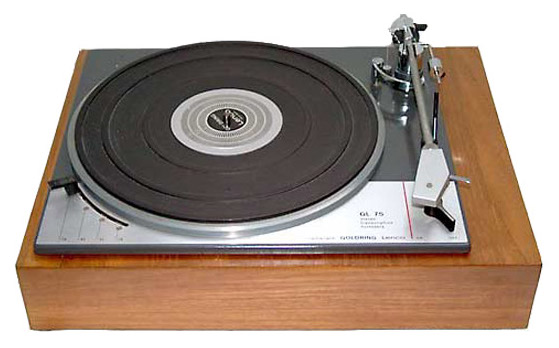
\includegraphics[width=0.25\textwidth]{assets/critical-review/Gramaphone.jpeg}
    \caption{Gramaphone}
    \label{fig:critical-review:Gramaphone}
\end{wrapfigure}
De grammofoonplaat is een iteratie op de wasrol. In plaats van een ronde rol is het geluid bij de grammofoon opgeslagen op een platte plaat. Het schrijven en afspelen werkte bij de eerste iteraties van de grammofoon nog steeds voornamelijk mechanisch en drukken per individuele plaat. In de latere iteraties van de grammofoonspeler werd meer elektronica verwerkt waardoor de kwaliteit en volume van het geluid beter werd, massaproductie mogelijk werd en het daarnaast ook mogelijk werd om de muziek in stereo af te spelen.

Een groot voordeel van de grammofoon is het medium waarop de muziek is opgeslagen: een plaat ten opzichte van de wasrol. Platen zijn makkelijker te massa-produceren omdat ze gedrukt kunnen worden vanuit een mal. Een wasrol moet individueel worden beschreven en kan hierdoor niet makkelijk in grote hoeveelheid geproduceerd worden. Platen zijn daarnaast ook makkelijker in opslag omdat ze plat zijn. Door het gebruik van vinyl bij latere platen blijven ze ook langer goed.

Net als de wasrol heeft een plaat een maximale speelduur vanwege zijn formaat. Door technische restricties van verschillende soorten spelers zijn standaarden ontstaan voor de lengte van platen. De eerste generatie grammofoonplaten hadden door hun formaat (30cm, 12"), naalddikte en toerental van 78rpm een maximale speelduur van ongeveer 5 minuten. Het toerental komt voort uit een optimale geluidskwaliteit bij de afstand tussen de groeven van een 12" plaat, en het gebruik van standaard naainaalden. Door technische verbeteringen werd het vanaf 1950 mogelijk om platen met steeds langere speeltijd te drukken. 

De speelduur en snelheid zijn door de jaren heen een standaard geworden. Deze standaarden worden tegenwoordig nog steeds aangehouden, ondanks dat dit vanwege de nieuwe technologieën niet meer nodig is. Albums zijn tegenwoordig vaak nog steeds rond 40 minuten lang. Dit is een interessant gegeven omdat het laat zien dat de technische beperkingen van een medium de manier waarop muziek wordt geschreven kan beïnvloeden. De NichePlayer heeft als creatief platform het doel om juist geen beperkingen op te leggen aan de muziek die erop wordt gepubliceerd. Er is geen maximale lengte van een nummer of album, afgezien van de beschikbare opslagruimte van de server. Daarnaast wordt op veel plekken in het proces de vrije keuze van de artiest benadrukt.

Hoewel de technologie van vinyl spelers al lange tijd achterhaald is blijft het een populair medium. Volgens een onderzoek van de RIAA \citep{year_end_2022_RIAA_revenue_statistics} was de omzet van de verkoop van vinyl in de VS in 2022 hoger dan dat van de CD. Er werden dat jaar rond de 41 miljoen platen verkocht met een totale waarde van \$1.2 miljard dollar tegenover 33 miljoen CD's ter waarde van \$483 miljoen dollar. Het is opvallend dat vinyl een beter verkocht medium is in deze tijd. De CD is qua geluidskwaliteit vele malen beter dan vinyl, is kleiner en makkelijker af te spelen.

Het is bijzonder dat de LP nog steeds in deze hoeveelheden verkocht wordt. Een mogelijke verklaring is dat het bij de LP niet meer gaat om het geluid, maar om het bezitten van het object. Een LP is een hiermee een verzamelobject geworden en wordt vaak gekocht door mensen die de muziek al digitaal hebben.

De NichePlayer kan een rol in spelen in de fysieke verkoop door het mogelijk te maken om een fysiek object te koppelen aan een digitaal album. Wanneer het fysieke object wordt gekocht kan de muziek ook digitaal worden aangeboden aan de luisteraar. Dit kan een manier zijn om de fysieke verkoop van muziek verder te stimuleren.

Samenvattend is de LP relevant voor de NichePlayer omdat het een fysiek product is wat in massa verkocht werd. Daarnaast is het de laatste jaren meer een verzamelobject geworden en staat het los van het afspelen van muziek. De NichePlayer kan de verkoop van fysieke producten terugbrengen.

\subsubsection*{Cassette}
\begin{wrapfigure}{r}{0.25\textwidth}
    \centering
    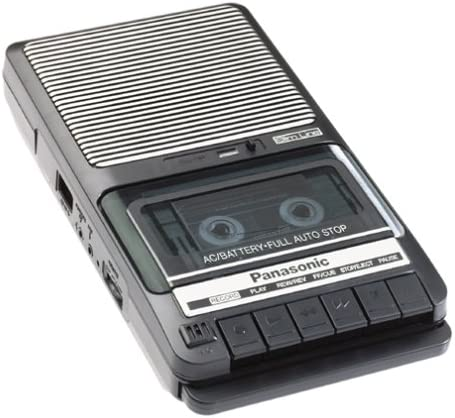
\includegraphics[width=0.25\textwidth]{assets/critical-review/Tape.jpg}
    \caption{Cassette recorder}
    \label{fig:critical-review:tape}
\end{wrapfigure}
Bij de cassette is het geluid opgeslagen op een magnetisch geladen strip. De strip is opgerold in een plastic behuizing, een cassette, en kan worden afgespeeld met een speciale speler. De cassettespeler rolt de strip af van de ene spoel naar de andere en leest de magnetische strip af met een leeskop. De signalen worden vervolgens versterkt en omgezet in geluid.

Een belangrijk voordeel van de cassette is dat het een medium is wat makkelijk meegenomen kan worden. De cassette is klein en gebruikt relatief eenvoudige technologie. Cassettespeler konden hierdoor erg klein worden gemaakt, en konden bovendien op batterijen werken. Dit maakte het vervolgens weer mogelijk om muziek mee te nemen en af te spelen op plekken waar geen elektriciteit is. Dit is een groot voordeel ten opzichte van de platenspeler. Platen zijn redelijk groot (30cm of 12"), waardoor ook de speler groot moet zijn.

Daarnaast is het ook mogelijk om zelf opnames te maken op een cassette. Het opnemen van muziek op een cassette is echter niet zonder kwaliteitsverlies. De magnetische strip is gevoelig voor ruis en de kwaliteit van de lees- en schrijfkop bepaald sterk de kwaliteit van het geluid. Het is niet mogelijk om een exacte kopie te maken van een cassette. Mensen konden zelf mixtapes maken van hun favoriete muziek, en deze vervolgens verdelen onder hun vrienden. Dit heeft een nieuwe cultuur gecreëerd rondom het medium die nog steeds zichtbaar is in sommige genres.

\begin{wrapfigure}{r}{0.25\textwidth}
    \centering
    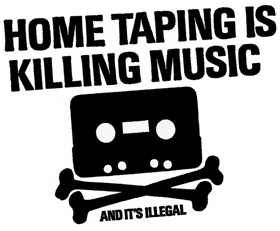
\includegraphics[width=0.25\textwidth]{assets/critical-review/Home_taping_is_killing_music.png}
    \caption{Home Taping is Killing Music}
    \label{fig:critical-review:home_taping_is_killing_music}
\end{wrapfigure}
Het kunnen opnemen op een cassettetape is echter niet altijd een gewenste functionaliteit. Het is hiermee namelijk mogelijk om bestaande muziek op te nemen van de radio, plaat of van een andere cassette, zonder hiervoor te betalen. Hiermee kunnen veel illegale kopieën worden gemaakt, ofwel piracy. In reactie hierop werden verschillend acties opgezet, waaronder de 'Home Taping is Killing Music' campagne \cite{bottomley2015home}. Waar een deel van de artiesten en de luisteraars blij waren met de nieuwe (vaak anarchistische) cultuur, waren de platenmaatschappijen hier niet blij mee. Ze waren bang dat door het kopiëren van muziek de verkoop van verkochte muziek zou dalen.

Het opnieuw opnemen van muziek is echter niet illegaal, zolang het maar voor eigen gebruik is. Dit gebruik is vastgesteld in de wetgeving van de meeste landen. Wanneer je een product hebt gekocht, mag je het gebruiken zoals je wilt, inclusief overzetten naar een ander medium. Het is echter niet toegestaan om de muziek te verkopen met commerciële doeleinden. 

Het logo van de 'Home Taping is Killing Music' campagne wordt nog steeds gebruikt, al is het niet voor dezelfde doeleinden. De torrentsite The Pirate Bay gebruikt het logo als een soort van trofee voor het downloaden van muziek. Het is een symbool geworden voor de strijd tussen de muziekindustrie en de luisteraar.

Cassettes zijn interessant voor de NichePlayer vanwege hun effect op de cultuur van muziek. Het is een medium dat makkelijk te verspreiden is en waarop mensen zelf muziek kunnen opnemen. Het is daarmee een creatief medium wat mensen in staat stelt om zelf muziek te maken en te verspreiden. De NichePlayer kan een rol spelen in het verspreiden van muziek door het mogelijk te maken om muziek op te nemen of te mixen en dit te kunnen delen met anderen.

\subsubsection*{CD}
\begin{wrapfigure}{r}{0.25\textwidth}
    \centering
    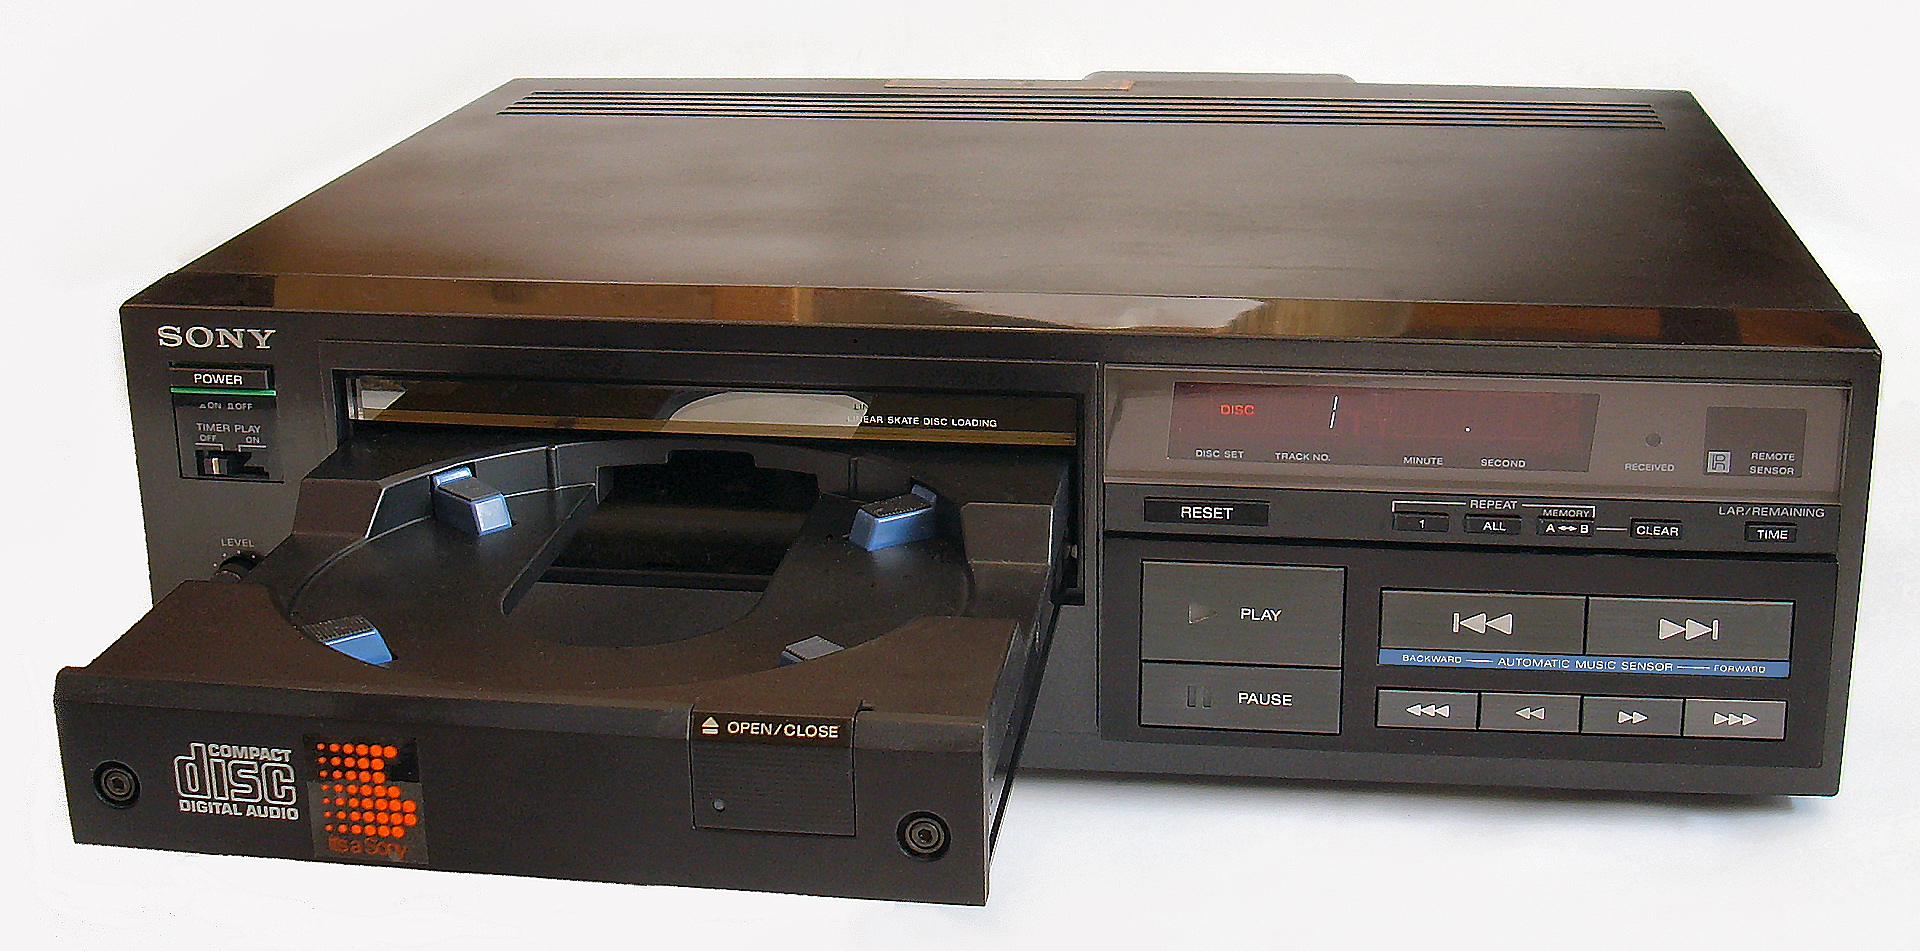
\includegraphics[width=0.25\textwidth]{assets/critical-review/CD-Player.jpeg}
    \caption{Eerste commerciële CD speler}
    \label{fig:critical-review:cp-player}
\end{wrapfigure}
De CD is het eerste volledig digitale medium. Net als de grammofoonplaat wordt het geluid opgeslagen op een schijf door middel van putjes. Bij een CD wordt echter geen gebruik gemaakt van een naald, maar wordt de diepte van de groef gelezen door een laser. De speler is daarbij ook veel kleiner dan een platenspeler omdat er weinig mechanisch onderdelen zijn, wat het makkelijker maakt om mee te nemen.

Het grote technische voordeel van de CD is de kwaliteit. Geluid op een CD wordt opgeslagen op 44.1 KHz sample rate en 16-bit bit diepte. Dit betekent dat frequenties tot 22.05 KHz kunnen worden opgeslagen, wat een veel hogere kwaliteit is dan de cassette en de grammofoonplaat. Gemiddelde cassette bandjes hadden een frequentie bereik tot 12 KHz \citep{van1970audio}, en de grammofoonplaat tot 15 KHz. Daarnaast is de ruisvloer van de CD significant lager dan zijn voorgangers.

De geluidskwaliteit van een CD gaat daarnaast niet verloren na verloop van tijd. Wanneer een plaat vaak wordt afgespeeld is er een kans dat de groeven gaan vervormen. Dit komt voornamelijk omdat de naald door de groeven van de lp schuurt, wat warmte opwekt. Omdat een CD met een laser wordt uitgelezen in plaats van een naald is er geen fysiek contact met de schijf waardoor dit geen probleem is. Een CD kan echter nog steeds wel beschadigd raken door krassen of vuil. In plaats van de geluidskwaliteit die achteruit gaat, zal de CD dan stukken overslaan of helemaal niet meer af te spelen zijn.

Net als de cassette is het mogelijk om zelf CD's te branden. Bij een CD is het echter wel mogelijk om een exacte kopie te maken van een CD. Beginnende artiesten konden hiermee zelf CD's branden en deze verkopen of weggeven tijdens optredens. Dit was een goede manier om de muziek te verspreiden en om fans te krijgen.

Ondanks dat de cd industrie strenge controles deed op zijn werknemers en de productie van CD's gebeurde het toch vaak dat CD's werden gelekt. Deze werknemers kopieerden de CD's en maakte hier vervolgens op eigen CD branders kopieën van, die ze vervolgens verkochten op straat. Dit werd ook wel bootlegging genoemd. De kwaliteit van deze CD's was exact hetzelfde als het origineel. Een nadeel was echter wel dat de branders erg duur waren en dat de snelheid van de branders in die tijd nog niet zo hoog was, waardoor het branden van een CD lang kon duren. Hierdoor was het bootleggen van CD's niet altijd een winstgevende business.

De CD industrie was enorm. Tijdens de piek van de CD industrie in 2000 werden er in de Verenigde Staten meer dan 942.5 miljoen CD's verkocht ter waarde van \$13.2 miljard dollar \citep{riaa2022salesdatabase}. Toch is het interessant om te zien dat steeds minder mensen tegenwoordig cd spelers in huis hebben.

Het verdwijnen van een speler is niet nieuw, toen de CD werd geïntroduceerd was het ook niet meer nodig om een cassette spelers in huis te hebben. CD en DVD spelers zaten echter wel in veel verschillende soorten apparaten, van home-audio systemen tot computers. Naast het afspelen van muziek was het ook een bekende data-drager waarop bijvoorbeeld software werd geleverd. Het verdwijnen van de CD en CD speler is een interessante ontwikkeling omdat het laat zien dat een medium niet altijd relevant blijft, en daarnaast ook niet altijd toegankelijk.

De CD is om meerdere redenen interessant voor de NichePlayer. Het was het eerste medium waarbij artiesten zelf muziek konden uitbrengen met goede kwaliteit. Daarnaast is het goed om rekening te houden met de mogelijkheid tot kopiëren van de muziek. Verder is het zonde dat muziek niet meer kan worden afgespeeld als een medium 'uit de mode' raakt. Internet is een medium wat veel breder is, en daardoor ook veel langer relevant blijft. Door manieren te vinden waarop de muziek online kan worden blijven aangeboden (ook als het bedrijf failliet is) kan het altijd worden afgespeeld, ongeacht het medium waarop het wordt afgespeeld.

\subsubsection*{MP3 en Internet}
\begin{wrapfigure}{r}{0.25\textwidth}
    \centering
    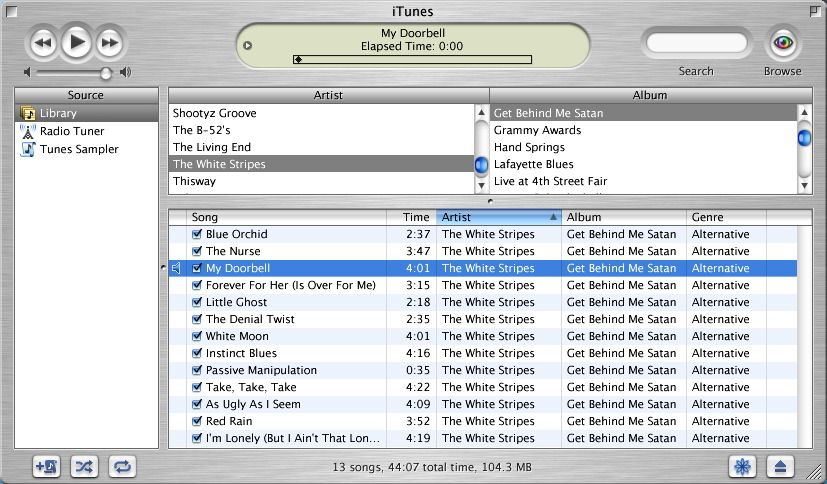
\includegraphics[width=0.25\textwidth]{assets/critical-review/iTunes_v1.jpeg}
    \caption{iTunes}
    \label{fig:critical-review:iTunes}
\end{wrapfigure}

Internet heeft een grote impact gehad op de muziekindustrie. Dit was vooral mogelijk door de uitvinding van de MP3.

Het boek How Music got Free, geschreven door Stephen Witt \citep{HowMusicGotFree} geeft een overzicht van de opkomst van de MP3, internet en hub invloed op de muziek industrie. Dit wordt gedaan vanuit verschillende oogpunten: de ontwikkelaars van de MP3, de muziek industrie en de piraten. 

\paragraph*{MP3}
Met de komst van grotere harde schijven en computers met CD spelers werd het mogelijk om muziek te rippen van een CD. Dit is het proces waarbij de muziek van een CD wordt gekopieerd naar een computer en wordt opgeslagen op de harde schijf. Toch was het niet mogelijk om de volledige kwaliteit van de CD op te slaan, omdat de harde schijven in die tijd niet groot genoeg waren (CD's hebben een maximale opslag van 700mb). Dit veranderde met de uitvinding van de MP3, een compressie formaat voor audio die bestanden 4x kleiner kan opslaan met minimaal kwaliteitsverlies. Hierdoor werd het mogelijk om muziek op te slaan op eigen computers, waardoor de CD niet meer nodig was om af te spelen. 

Door de MP3 konden bestanden veel makkelijker vanaf het internet worden gedownload. Op verschillende internet kanalen (IRC, forums en andere diensten uit die tijd) werden download links aangeboden waar muziek kon worden gedownload. De kwaliteit van deze download was exact bit-perfect aan het origineel wat was geüpload. Dit was een grote verandering ten opzichte van de cassette, waarbij de kwaliteit van de kopie altijd minder was dan het origineel.

\paragraph*{Torrents en Peer2Peer}
Naast IRC en forums werden er ook andere technologieën ontwikkeld die niet afhankelijk waren van servers. Peer 2 Peer is een technologie waarbij computers direct met elkaar kunnen communiceren, waardoor het  mogelijk is om bestanden te delen zonder dat er een centrale server nodig is. Een bekend voorbeeld hiervan is Napster, een programma wat speciaal was ontwikkeld voor het uitwisselen van muziek. Op zijn piek had Napster 80 miljoen gebruikers \citep{gown2002requiem}. De dienst werd echter snel verbonden met copyright schending. Dit leidde uiteindelijk op juli 11 2001 tot het stoppen van de dienst.

Naast Napster werden ook andere technologieën ontwikkeld, namelijk BitTorrent. Net als Napster wordt verbinding gemaakt tussen meerdere computers, en worden hiermee bestanden uitgewisseld. Een verschil met Napster is dat Bittorrent van meerdere computers tegelijk zijn bestanden ophaalt. Hierdoor gaat het downloaden veel sneller. BitTorrent heeft daarnaast niet één zoekmachine, maar biedt de mogelijkheid om zelf een zoekmachine te maken. Een Torrent bestand heeft vervolgens de informatie over de bestanden die worden gedeeld, en hoe deze kunnen worden opgehaald. De zoekmachine heeft hiermee geen controle over wat er op het platform wordt aangeboden, en daarnaast ook niet de bestanden zelf. Omdat de zoekmachines puur werken als een index, en niet als een host, is het moeilijk om de site offline te halen.

Torrents zijn legaal gezien een grijs gebied. Het is niet illegaal om een torrent bestand te downloaden, maar wel bestanden die copyright hebben te delen. Aangezien binnen het torrent protocol iedereen tegelijkertijd download en upload, is het niet mogelijk om alleen te downloaden. Het is daarbij wel mogelijk om te controleren wie er precies upload door de peer-lijst met IP adressen op te slaan.

Een nadeel van Napster en Torrent was dat het downloaden van de bestanden nog erg lang duurde doordat het internet nog niet snel was. Omdat de bestanden niet vooraf geluisterd konden worden gebeurde het dan ook vaak dat een verkeerde versie, of een versie met lage kwaliteit werd gedownload waar dan heel lang op was gewacht.

Napster en torrent zijn ontwikkeld als showcase van technologie, en hadden daarbij geen illegale intenties. Het was een manier om te laten zien wat er mogelijk was met de technologie van die tijd. De content die op de diensten terecht kwam had weinig te maken met de ontwikkelaars.

\paragraph*{iTunes}
Om de steeds meer groeiende muziek bibliotheek te ordenen en af te spelen werd software zoals iTunes ontwikkeld. Deze muziekspeler indexeert alle (mp3) files op de harde schijf en maakt het mogelijk om hierin te zoeken en af te spelen. 

Een probleem was dat de muziek die werd gedownload een legaal randgeval was. Het is namelijk niet illegaal om muziek te downloaden en te rippen van een CD, maar wel om deze te uploaden en te verspreiden. Met vorige media bleef het origineel belangrijk omdat bij iedere kopie de kwaliteit sterk omlaag ging, maar aangezien digitale kopieën bit-perfect zijn is het origineel niet meer nodig. Het is hierdoor mogelijk om CD's te drukken van zo'n kopie, en deze vervolgens te verkopen.

\begin{quotation}
    Even though mp3 files, a compressed form of digital signals, are inferior in audio quality to the original digital version, the fact that they too can be copied indefinitely with perfect accuracy, further intensifies the debate. Everyone owns the original, and the propriety of ownership is no longer bounded by physical laws, only by legal statutes.
    \citep{lansky2004importance}
\end{quotation}

In 2002 werd de iTunes Music Store geïntroduceerd \citep{chen2010itunes}. Via deze webwinkel kon muziek legaal worden gekocht en daarna gedownload. De muziek was in eerste instantie alleen beschikbaar in AAC en was met DRM (Digital Rights Management) beveiliging. Dit betekent dat de muziek alleen kon worden afgespeeld op een computer waarop de muziek was gekocht. Dit was een grote stap voorwaarts in de muziekindustrie, omdat het hiermee mogelijk werd om muziek legaal te kopen en te downloaden. In 2009 werd de DRM beveiliging verwijderd, waardoor de muziek op ieder apparaat kon worden afgespeeld.

Door de digitale toegang van de muziek hoefde niet meer een heel album gekocht te worden, maar konden mensen ook losse nummers kopen en downloaden. Mensen konden luisteren naar een preview van 30 of 90 seconden, net als ze zouden doen in de platenzaak. Het kopen van enkele nummers was een grote verandering ten opzichte van de voorgaande media, waarbij altijd een heel album moest worden gekocht.

Vanwege de komst van de MP3 en het internet werd het voor het eerst mogelijk om muziek te verkrijgen zonder dat daar een fysiek medium voor nodig was. Daarbij werd de beschikbaarheid van de muziek ook veel groter. Een harde schijf heeft altijd een zelfde fysieke grote, ongeacht hoeveel muziek erop staat. Dit was een grote verandering ten opzichte van de voorgaande media, waarbij altijd een fysiek medium nodig was om muziek af te spelen. Dit heeft geleid tot een grote verandering in de muziekindustrie, waarbij voor het eerst de fysieke verkoop van muziek sterk afnam.

% Relevantie NichePlayer
Door de uitvinding van internet en de MP3 wat het voor het eerst mogelijk muziek af te spelen zonder een fysiek medium. Het heeft hiermee de muziekindustrie volledig op zijn kop gezet. De NichePlayer probeert een aantal veranderingen die door de komst van internet zijn ontstaan terug te draaien, waaronder het bezitten van een fysiek product, en het faciliteren van beperkte oplagen.

\subsubsection*{Streaming}
\begin{wrapfigure}{r}{0.25\textwidth}
    \centering
    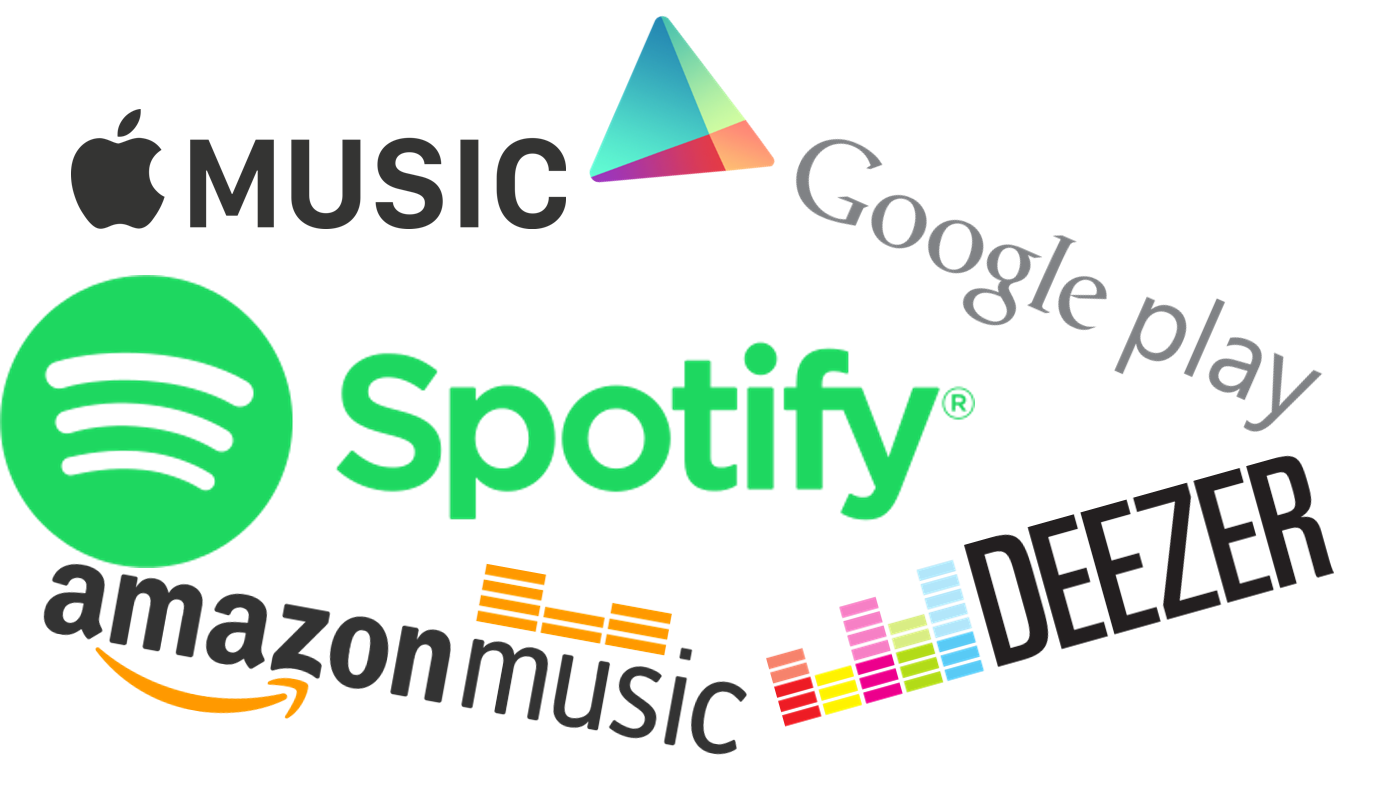
\includegraphics[width=0.25\textwidth]{assets/critical-review/StreamingServices.png}
    \caption{Streaming services}
    \label{fig:critical-review:StreamingServices}
\end{wrapfigure}

Het meest recente medium is Muziek Streaming. Spotify was in 2021 met een marktaandeel van 30.5\% met voorsprong de grootste streamingdienst ter wereld \citep{mulligan2022marketshares}.

Streamingdiensten zijn grote databases aan muziek. In plaats van een eigen, beperkte, hoeveelheid muziek heeft de luisteraar een vrijwel onbeperkte toegang. De muziek wordt gestreamd en is direct af te spelen op het apparaat met bijna geen vertraging. Er is hierbij geen opslagruimte nodig omdat de muziek niet wordt opgeslagen op het apparaat.

In tegenstelling tot vorige media wordt er bij de meeste streamingdiensten niet betaald per album of nummer. In plaats daarvan betaald de luisteraar een vast bedrag per maand. Het totaalbedrag van alle abonnementen wordt vervolgens verdeeld over artiesten op basis van hoe vaak een nummer is afgespeeld. Een consequentie hiervan is dat de luisteraar geen eigenaar is van de muziek, maar betaald voor toegang tot de muziek. Wanneer het abonnement wordt opgezegd is de muziek niet meer beschikbaar. 

Streaming heeft het luistergedrag en de muziek zelf significant veranderd. Binnen streamingdiensten kunnen luisteraars playlists aanmaken met hun favoriete nummers. Deze playlists kunnen vervolgens worden gedeeld met andere luisteraars. Daarnaast maken curators van de streamingdiensten ook playlists. De verschuiving waarbij de focus meer ligt op lossen nummers die begon bij het opkomen van muziek winkels via internet werd hiermee versterkt. Daarnaast is het met streaming veel makkelijker om losse nummers te publiceren.

Door het algoritme van spotify waarmee het luistergedrag wordt opgeslagen heeft de muziek veranderd. Omdat een stream pas meegerekend wordt wanneer hij meer dan 30 seconden is afgespeeld verplaatsen artiesten de drop of hook van een nummer steeds verder naar achteren. Daarnaast lijken nummers korter te worden, zodat ze vaker worden afgespeeld.

Streaming is alleen mogelijk door de groei binnen het internet. Het is belangrijk binnen streaming dat de muziek vrijwel direct en zonder buffering wordt afgespeeld. Een streamingdienst als Spotify maakt gebruik van verschillende trucs in het TCP/IP protocol van internet om de muziek zo snel mogelijk af te spelen. Hierbij wordt de data in heel veel kleine pakketjes verzonden. In tegenstelling tot normaal internet wordt een pakket wat niet aankomt genegeerd. Dit is niet erg omdat de data die mist niet direct hoorbaar is en de muziek alsnog kan worden afgespeeld. Daarbij is dit alleen noodzakelijk bij het begin van het nummer, omdat de muziek daarna al is opgeslagen in een buffer. Door deze techniek is het mogelijk om muziek te streamen met een zeer lage latency.

De NichePlayer is in praktijk hetzelfde als bestaande streamingdiensten. Er is een online database aan muziek die de gebruiker kan afspelen wanneer er wordt betaald. De muziek is direct af te spelen zonder het eerst te downloaden. Het verschil ligt echter in het businessmodel. Artiesten krijgen veel meer de vrijheid om hun inkomsten model te bepalen. Daarnaast is het mogelijk om fysieke producten te koppelen aan de muziek waardoor het bezitten van muziek weer belangrijk wordt.

% ---------------------------------------------------------------------------------------- %
\subsection{Concurrerende projecten}
\subsubsection*{TapTapes}
\begin{wrapfigure}{r}{0.25\textwidth}
    \centering
    
\includegraphics[width=0.25\textwidth]{assets/critical-review/TapTapes.png}
    \caption{TapTapes}
    \label{fig:critical-review:TapTapes}
\end{wrapfigure}
De NichePlayer is niet alleen in zijn soort. Er zijn veel vergelijkbare producten die het in de inleiding benoemde probleem proberen op te lossen. Een van deze diensten is TapTapes, een start-up uit Saarbrücken, Duitsland. Toevallig is dit het bedrijf waar ik in mijn bachelor stage heb gelopen. Het concept van de NichePlayer bestond toen al enkele jaren, maar heeft door de stage meer vorm gekregen.

TapTapes is een commercieel bedrijf dat een dienst aanbiedt om muziek te luisteren waarbij toegang wordt gegeven met een fysieke kaart. Net als de NichePlayer moet deze kaart gescand worden door een telefoon om te koppelen aan het apparaat.

Het grote verschil tussen TapTapes en de NichePlayer is dat bij de TapTapes een overeenkomst tussen de artiest en TapTapes nodig is. TapTapes drukt namelijk de kaarten  en koppelt deze met het systeem voor beveiligde toegang. Daarnaast moet de software momenteel door TapTapes ingericht worden wat betreft uiterlijk en inhoud. Dit is een groot verschil met de NichePlayer, waarbij de artiest zelf de kaarten kan maken en de muziek kan koppelen. In het basispakket van de NichePlayer ben ik als bedrijf zelfs helemaal niet betrokken, en kan de artiest alles zelf doen. Het businessmodel van de NichePlayer is gebaseerd op het aanbieden van extra diensten, waarmee de ervaring van de luisteraar kan worden verbeterd.

Tijdens het ontwikkelen van de NichePlayer moet ik constant in de gate houden dat het concept en de uitwerking niet te veel op TapTapes gaat lijken. Dit is lastig omdat ik nog steeds een van de hoofdontwikkelaars ben bij TapTapes. Het is belangrijk om hier goed over te blijven communiceren met de eigenaar van TapTapes.

\subsection{NichePlayer}
\begin{wrapfigure}{r}{0.25\textwidth}
    \centering
    
\includegraphics[width=0.25\textwidth]{assets/critical-review/NichePlayer.png}
    \caption{NichePlayer}
    \label{fig:critical-review:NichePlayer}
\end{wrapfigure}

% - Korte geschiedenis van de NichePlayer (vorige iteraties)
Er zijn in de afgelopen jaren veel iteraties geweest van de NichePlayer. Waar de ontwikkeling in 2014 begon als een simpele muziek player voor eigen gebruik (ik had toen geen Spotify maar wel een enorme muziekbibliotheek) is het nu uitgegroeid tot een product dat door iedereen te gebruiken moet gaan zijn. Het ontwikkelen van de NichePlayer is de rode draad geweest van mijn programmeer-ontwikkeling. In iedere iteratie is mijn groei op het gebied van software-development duidelijk te zien. Waar ik in de eerste iteraties alles zelf ontwikkelde ben ik later overgegaan naar het gebruik van libraries en frameworks. Ook is de code steeds beter georganiseerd en is de kwaliteit steeds beter geworden.

De NichePlayer is een streamingdienst die speciaal wordt ontworpen met creativiteit, openheid en transparantie in gedachte. Door de NichePlayer te gebruiken krijgt de artiest controle terug over het medium in de vorm van inkomsten en layout. De gebruiker krijgt de mogelijkheid om de artiest te steunen door middel van fysieke verkoop gekoppeld aan toegang tot de muziek. 

De NichePlayer is ontwikkeld voor kleine en beginnende artiesten. De NichePlayer zal dan ook niet gaan concurreren met bestaande diensten, simpelweg omdat deze concurrentie niet kan worden gewonnen.

\subsubsection*{Laatste iteratie (Bachelor SN)}
De laatste significante iteratie van de NichePlayer was ontwikkeld als afstudeerproject van mijn bachelor Muziek en Technologie. Bij deze versie gebruikte ik voor het eerst een backend framework (Symfony) en een frontend framework (VueJS). Dit was een grote stap voorwaarts in de ontwikkeling van de NichePlayer. Het gebruik van deze frameworks zorgde ervoor dat de code beter georganiseerd was en dat de ontwikkeling sneller ging. Het Supportive Narrative van mijn bachelor heb ik daarbij voornamelijk gebruikt om mijn proces te beschrijven en de keuzes voor technologieën te verantwoorden.

De reden dat dit niet de laatste iteratie is geworden voor productie is omdat het systeem softwarematig niet goed werkte. Het was niet mogelijk om met meer dan twee gebruikers tegelijk naar muziek te luisteren. De API werd niet correct aangeroepen en was daarbij ook niet goed geconfigureerd waardoor deze erg traag werkte. Ik gebruikte zelf ontwikkelde code om de frontend en de backend te laten communiceren en maakte niet gebruik van softwaretechnieken als relational mapping, caching en server-side filtering. Voor een prototype was dit geen probleem, maar voor een productieversie moet een systeem stabiel zijn en snel werken.

Daarnaast was de plek waar het systeem draaide een grote bottleneck. De backend draaide volledig in een virtuele server met weinig optimalisatie, en de data moest door verschillende computers heen om uiteindelijk bij de gebruiker te komen. Dit zorgde ervoor dat de backend niet goed bereikbaar was en dat de API niet goed werkte.

\subsubsection*{Nieuwe iteratie noodzakelijk}
% - Verschil met vorige iteraties NichePlayer, waarom was een nieuwe iteratie nodig?
Deze hiervoor genoemde problemen konden niet meer worden opgelost binnen de bachelor iteratie omdat het voornamelijk aan de core van het systeem lag. Daarom heb ik besloten om een nieuwe iteratie te starten waarbij deze problemen worden opgelost. Het concept blijft hierbij hetzelfde, en ook de libraries van de back- en frontend worden hergebruikt. Er worden echter wel nieuwe plugins toegevoegd waaronder een Object Relation Mapping plugin en een plugin voor communicatie met de API. De code wordt opnieuw geschreven volgens moderne syntax standaarden wat wordt geforceerd binnen mijn code-editor door middel van een extensie.

Object Relation Mapping is een manier om data aan elkaar te koppelen. Een gebruiker heeft bijvoorbeeld meerdere albums, en een album heeft meerdere nummers. Door gebruik te maken van ORM hoeft de programmeur niet zelf de data aan elkaar te koppelen, maar wordt dit automatisch gedaan. Dit zorgt ervoor dat de code minder complex is en dat er minder fouten gemaakt kunnen worden. Daarnaast is het met een ORM plugin makkelijker om een relatieveld van een object op te vragen (bijvoorbeeld het album van een nummer).
